\documentclass[10pt,a4paper]{moderncv}
\moderncvtheme[blue]{casual}
\usepackage{lmodern}
\usepackage[ngerman]{babel}
\usepackage{amsmath}
\usepackage[utf8]{inputenc}
\usepackage{textcomp} % for Euro symbol

% Micro typography (especially space settings)
\usepackage{microtype}

\usepackage[absolute]{textpos}

% The borders are EXTREMELY big, so scale everything down by 20 percent.
\usepackage[scale=.9]{geometry}
\setlength{\hintscolumnwidth}{5cm}

% Set nice font.
%\usepackage[semibold]{crimson}
%\usepackage[sb]{libertine}
%\usepackage{mathpazo}
\usepackage{charter}

% Set Reg and TM symbols and XeonPhi command, for ease-of-use
\def\SymReg{\textsuperscript{\textregistered}}
\def\SymTM{\textsuperscript{\texttrademark}}
\newcommand{\XeonPhi}{Intel\SymReg Xeon Phi\SymTM\,}

\def\Euro{€}

% Personal data. At least that should be clear.
\name{Dr. Thomas}{Lang}
\title{Curriculum Vitae}
\address{Brunnengasse 26/4}{4792 Münzkirchen}
%\phone{+43~(0)660/7333301}
\email{thomas.lang@iis.fraunhofer.de}
\social[twitter]{LangThomas93}
%\social[github]{langthom}
\social[linkedin][https://www.linkedin.com/in/thomas-lang-471692226/]{thomas-lang}
  
\begin{document}
\begin{textblock}{30}(10,2)
 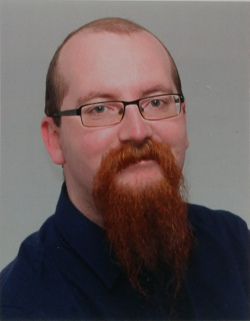
\includegraphics[width=90pt]{LangThomas.jpg}
\end{textblock}
\maketitle
\vspace{-1cm}
\section{Personal Information}
\cventry{Born}{20\textsuperscript{th} April 1993}{Schärding}{}{}{}
\cventry{Citizenship}{Austria}{}{}{}{}
\cventry{Confession}{Roman catholic}{}{}{}{}

\section{Education}
\subsection{PhD}
\cventry{04/01/2018 -- 04/14/2021}{University of Passau}{Computer Science}{Final grade $1.0$ (\emph{summa cum laude})}{}{}
\cventry{07/09/2021}{\textnormal{Thesis defence}}{}{}{}{}

\subsection{Study}
\cventry{Term 2016/17--Term 2017/18}{University of Passau}{Master Computer Science}{Final grade $1.1$ (with distinction)}{}{}
\cventry{Term 2013/14--Term    2016}{University of Passau}{Bachelor Computer Science}{Final grade $1.8$ (good)}{}{}

\subsection{School}
\cventry{2012}{Matura}{Average grade $1.2$ (with distinction)}{}{}{}
\cventry{2007--2012}{Höhere Technische Lehranstalt Innviertel-Nord in Andorf}{}{}{}{}
\cventry{2003--2007}{Hauptschule Münzkirchen}{}{}{}{}
\cventry{1999--2003}{Volksschule Münzkirchen}{}{}{}{}

\subsection{PhD Thesis}
\cventry{Title}{AI-Supported Interactive Segmentation of 3D Volumes}{}{}{}{}
\cvitem{Description}{Development of novel and general methods for interactive segmentation of very large 3D volumetric data using geometric information.}{}{}{}{}
\cvitem{Download}{\link{https://nbn-resolving.org/urn:nbn:de:bvb:739-opus4-9221}}{}{}{}{}

\subsection{Masters Thesis}
\cventry{Title}{Improving the Efficiency of Code Generation Based on Cylindrical Algebraic Decomposition}{}{}{}{}
\cvitem{Description}{Implementation and optimization of code generation for arbitrary loop bounds based on a cylindrical algebraic decomposition.}{}{}{}{}
\cvitem{Download}{\link{http://www.infosun.fim.uni-passau.de/cl/arbeiten/lang-m.pdf}}{}{}{}{}

\subsection{Bachelors Thesis}
\cventry{Title}{An \XeonPhi Backend for the ExaStencils Code Generator}{}{}{}{}
\cvitem{Description}{Extension of the ExaStencils code generator to support the \XeonPhi co-processor.}
\cvitem{Download}{\link{http://www.infosun.fim.uni-passau.de/cl/arbeiten/lang-b.pdf}}

\subsection{Language Skills}
\cvlanguage{German}{Native}{}
\cvlanguage{English}{Fluent}{}
\cvlanguage{Russian}{Fundamental}{}

\section{Presentations}
\cvitem{C++ course}{Presenter of a C++ course at the University of Passau, Winter terms 2018/19 and 2019/20}
\cvitem{PhD}{Several presentations throughout the doctorate}
\cvitem{Rigorosum}{PhD thesis defence presentation, 07/09/2021}

\clearpage

\section{Experience}
\subsection{Professional}
\cventry{09/01/2021 -- \phantom{08/31/2023}}{Post-Doc}{Fraunhofer IIS, Division EZRT/CTMT, Passau}{}{}{}{}
\cventry{04/01/2018 -- 08/31/2021}{Researcher}{Institute FORWISS, University of Passau}{}{}{}{}
\cventry{08/01/2016 -- 03/31/2018}{Student researcher}{Institute FORWISS, University of Passau}{}{}{}
%\cventry{01. 04. 2016 -- 30. 04. 2016}{HiWi}{Lehrstuhl für Schulpädagogik, Universität Passau}{}{}{}
%\cventry{15. 01. 2016 -- 15. 03. 2016}{HiWi}{Lehrstuhl für theoretische Informatik, Universität Passau}{}{}{}
%\cventry{01. 11. 2015 -- 30. 11. 2015}{HiWi}{Lehrstuhl für Informatik: Schwerpunkt Programmierung, Universität Passau}{}{}{}
%\cventry{15. 07. 2015 -- 14. 08. 2015}{HiWi}{Lehrstuhl für theoretische Informatik, Universität Passau}{}{}{}
%\cventry{04. 06. 2013 -- 30. 08. 2013}{Ferialarbeiter}{GST Global Sports Technologies GmbH}{}{}{}
%\cventry{11. 07. 2011 -- 26. 08. 2011}{Ferialarbeiter}{GST Global Sports Technologies GmbH}{}{}{}
\cventry{2015/2016}{Student researcher}{University of Passau, several chairs}{}{}{}
\cventry{07--08 / \{2011,2013\}}{Summer job}{GST Global Sports Technologies GmbH}{}{}{}

\subsection{Additional Qualifications}
\cvlistitem{Extensive experience with programming in \texttt{C/C++}, \texttt{Python}, \texttt{Haskell}}
\cvlistitem{Extensive experience with parallel programming (\texttt{OpenMP, MPI, GPU})}
\cvlistitem{Extensive experience with \LaTeX}
\cvlistitem{Extensive experience with machine learning techniques and their usage}
\cvlistitem{Experience with version control software (\texttt{git, svn})}

\section{Projects}
\subsection{Acquired projects}
\cventry{09/01/2021 -- 08/31/2022}{OntoSeg}{Efficient ontology-based segmentation of large volumes}{Budget: 90k\Euro}{}{}

\subsection{Project work}
\cventry{01/01/2022 -- \phantom{09/30/2025}}{QuaST}{Quantum-enabling Services und Tools f{\"u}r industrielle Anwendungen}{}{}{}
\cventry{01/01/2022 -- \phantom{09/30/2025}}{QACI}{Munich Quantum Valley - Quantum algorithms for application, cloud and industry}{}{}{}
\cventry{01/01/2022 -- \phantom{09/30/2025}}{Bay\@QS}{Research with applications of Quantum Computing}{}{}{}
\cventry{03/01/2021 -- 07/30/2021}{BM18}{High resolution industrial tomography beamline for large objects}{}{}{}
\cventry{04/01/2018 -- 02/28/2021}{Big Picture}{de.: Digitalisierung, Verarbeitung und Analyse kultureller und industrieller Objekte: Wertschöpfung aus großen Daten}{}{}{}

\section{Awards and Certificates}
\cvitem{11/11/2022}{Dissertationspreis der Universit{\"a}t Passau - Dissertation price of the University of Passau}
\cvitem{10/01/2019}{iSAQB~\textsuperscript{\textregistered} Certified Professional for Software Architecture - Foundation Level}
\cvitem{05/22/2018}{Professional Scrum Master I}2
\cvitem{01/26/2018}{msg Price for exceptional study work}


\section{Military Service}
\cvitem{Type}{Community Service}
\cvitem{Institution}{Lebenshilfe Münzkirchen}
\cvitem{Field of Work}{Aiding the care of care-dependent persons}
\cvitem{Duration}{08/01/2012 to 04/30/2013}

\section{Hobbies and Interests}
\cvitem{Computer Science}{Interest in software development with focus on machine learning, programming languages and image processing}
\cvitem{Genealogy}{Creation of a genealogy of my family}
%\cvitem{Buchbinden}{Erstellung von Büchern aus ehemals abonnierten Zeitschriften}
\cvitem{Origami}{Creation of complex origami figures}
\cvitem{Calligraphy}{Calligraphic writing, mostly in Kurrent}

\clearpage
\section{Publications}
{%
\renewcommand*{\bibliographyhead}[1]{}
\nocite{*}
\bibliographystyle{ieeetr}
\bibliography{publications}
}

\section{Scientific Activities}
\cvitem{2022}{Co-organizer of the 12\textsuperscript{th} Int. Conf. on Industrial Computed Tomography (iCT 2023)}


\vfill\makecvfoot{Münzkirchen,~\today}
\end{document}
